\chapter{Work Plan}

\label{Work_Plan}

\section{Stage 1}
Calibrate the models in \cref{fig: CM2pile} with partially observed Markov decision process.
\begin{figure}[H]
    \centering

    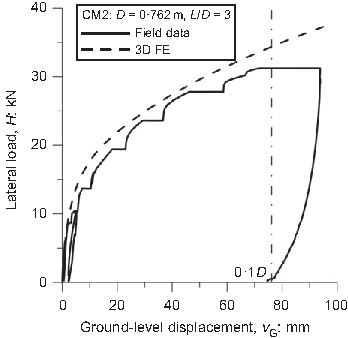
\includegraphics[width = 90mm]{Figures/figure-CM2.pdf}
    \caption{CM2 pile load displacement from \protect\cite{zdravkovic2020}}
    \label{fig: CM2pile}
\end{figure}

\begin{itemize}
    \item Software: ICFEP-Likelihoods and observed data.
    \item Constitutive model: clay in \cite{zdravkovic2020} and sand in \cite{taborda2020}.
    \item Consider the soil profile variance-Create the random field (scale of fluctuation in ICFEP).
\end{itemize}
Objective: Ensure the soil parameters in digital model can reveal unique characteristics of piles.

\section{Stage 2}
In operational Phase, Based on Partially observed Markov decision process method, continue the assimilation process: extend the digital twin capability to capture the piles response during loading.

\section{Stage 3}
Extension to Prediction




\section{Time plan}
\begin{table}[h]
\caption{PhD timeline}
\vspace{10pt}
\centering
\resizebox{\textwidth}{!}{
\begin{tabular}{|l|l|l|l|l|l|l|l|l|l|l|l|l|l|l|l|l|l|}
\hline
month                                                                           & 0 & 3                     & 6 & 9 & 12 & 15 & 18 & 21 & 24 & 27 & 30 & 33 & 36 & 39 & 42 & 45 & 48 \\ \hline
Literature review                                                               & \checkmark &\checkmark               &\checkmark   &   &    &    &    &    &    &    &    &    &    &    &    &    &    \\ \hline
\begin{tabular}[c]{@{}l@{}}Numerical modelling\\ (Data collection)\end{tabular} &   &\checkmark&  \checkmark & \checkmark  & \checkmark   &\checkmark    & \checkmark   &    &    &    &    &    &    &    &    &    &    \\ \hline
\begin{tabular}[c]{@{}l@{}}Statistics Methods \\ learning\end{tabular}          &   &\checkmark                       &\checkmark   & \checkmark  &\checkmark    & \checkmark   &   \checkmark &\checkmark    &\checkmark    &    &    &    &    &    &    &    &    \\ \hline
\begin{tabular}[c]{@{}l@{}}Statistics analysis\\ calibration\end{tabular}       &   &                       & \checkmark  &  \checkmark & \checkmark   &    &    &    &    &    &    &    &    &    &    &    &    \\ \hline
\begin{tabular}[c]{@{}l@{}}Statistics analysis\\ assimilation\end{tabular}      &   &                       &   &   &    &  \checkmark  &   \checkmark &\checkmark    &  \checkmark  & \checkmark   &\checkmark    &    &    &    &    &    &    \\ \hline
\begin{tabular}[c]{@{}l@{}}Statistics analysis\\ prediction\end{tabular}        &   &                       &   &   &    &    &    &    &    &    &   &  \checkmark  &   \checkmark &  \checkmark   &    &    &    \\ \hline
Thesis writing                                                                  &   &                       &   &   &    &    &    &    &    &    &    &    &    &    &     \checkmark&  \checkmark   & \checkmark    \\ \hline
Journal/Conference                                                              &   &                       &   &   &    &    &    &     \checkmark&    &    &    &    \checkmark &    &    &    &    &  \checkmark   \\ \hline
\end{tabular}}
\end{table}
